%
% pdeloesung.tex -- Loesungsprinzip für partielle Differentialgleichungen
%
% (c) 2018 Prof Dr Andreas Müller, Hochschule Rapperswil
%
\section{Lösungen von partiellen Differentialgleichungen%
\label{section:pdeloesungen}}
\rhead{Lösungen von partiellen Differentialgleichungen}
In diesem Kapitel haben wir Strömungen mit Hilfe partieller
Differentialgleichungen beschrieben.
Natürlich ist die Theorie der partiellen Differentialgleichungen viel
zu umfangreich, als dass in diesem Abschnitt eine Darstellung gegeben
werden könnte, die diesem Thema auch nur annährend gerecht wird.
Wir können bestenfalls hoffen, ein paar für unsere Zwecke wesentliche
Ideen zu vermitteln.
Für eine vollständigere Darstellung sei auf \cite{skript:pde}
oder \cite{skript:part-diff} verwiesen.

Die Funktionenräume, in denen die Lösungsfunktionen von Differentialgleichungen
zu finden sind, sind unendlich dimensional, was sehr erschwert,
dafür überhaupt eine Lösung zu finden.
Bereits bei der Lösung gewöhnlicher Differentialgleichungen hat man
gelernt, dass sich die Lösungsmenge durch einige wenige Integrationskonstanten
beschreiben lassen.
Bei partiellen Differentialgleichungen ist eine Lösungsfunktion von
mehrern Variablen gesucht.
Es wäre uns daher bereits geholfen, wenn wir sie durch
Funktionen parametrisieren könnten, die nur von wenigen Variablen
abhängen.
Im besten Fall können wir dann für diese Parameterfunktionen gewöhnliche
Differentialgleichungen aufstellen.
Auf diese Art und Weise erhalten wir in mehreren Schritten ein
endlichdimensionales Problem.

Das Ziel dieses Abschnittes ist daher, einige Methoden zusammenzustellen,
mit denen man ein allgemeines Problem über partielle Diffentialgleichungen
für Zwecke der Simulation oder Approximation
in ein endlichdimensionales Problem umwandeln kann.

\subsection{Diskretisation\label{section:diskretisation}}
Der einfachste Ansatz, partielle Differntialgleichungen zu lösen,
folgt den Verfahren, die auch für gewöhnliche Differentialgleichungen
\cite{skript:mathsem-dgl} 
zum Erfolg führen, nämlich sich auf die Berechnung von Funktionswerten
der Lösungsfunktion an diskreten Punkten des Definitionsgebietes zu
beschränken.
Zu diesem Zweck werden Ableitungen durch Differenzenquotienten ersetzt.
Wir illustrieren das Vorgehen an einigen Beispielen.

\subsubsection{Das Poisson-Problem}
\begin{figure}
\centering
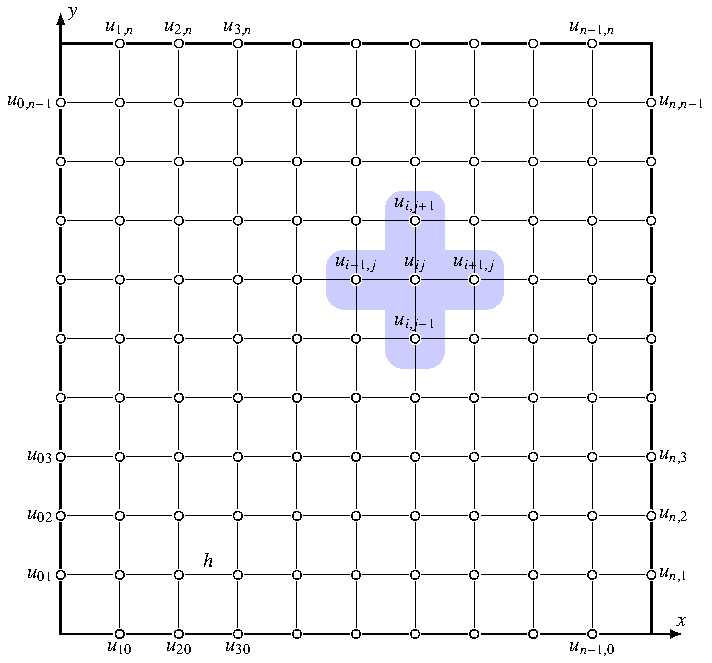
\includegraphics{chapters/2/poisson.pdf}
\caption{Diskretisation des Poisson-Problems
\label{skript:poisson:grid}}
\end{figure}
Wir suchen eine Lösung der Differentialgleichung
$\Delta u = 0$ auf dem Einheitsquadrat $\Omega=\{(x,y)\,|\, 0<x,y < 1\}$
mit den Randbedinungen $u(x,y)=g(x,y)$ für Punkte $(x,y)$ auf dem
Rand $\partial\Omega$.
\index{Poisson-Problem}%
Dies ist das Poisson-Problem.
Die allgemeine Theorie \cite{skript:pde} klassifiziert dieses Problem
als eine elliptische partielle Differentialgleichungen und erklärt,
dass das Poisson-Problem unter milden Annahmen über die Randwerte
eine eindeutig bestimmte glatte Lösung hat.
Sie liefert auch eine Methode, diese Lösung zu finden.

Für die numerische Lösung verwenden wir ein Gitter mit den Punkten
\[
P_{ij}
=
(x_i,y_j)
=
(ih, jh)
\qquad\text{mit}\qquad
i,j=0,\dots,n,\quad
h = \frac1n
\]
(siehe auch Abbildung~\ref{skript:poisson:grid}).
Die Punkte mit $i,j=0,n$ beschreibend den Rand.
Wir kürzen die Werte $u_{ij}=u(x_i,y_j)$ ab.
Die Randwerte sind bekannt, es gilt
\begin{align*}
u_{0j} &= g(0,jh)
&&\text{und}&
u_{nj} &= g(1,jh)
&&\text{mit $1\le j < n$}
\\
u_{i0} &= g(ih,0)
&&\text{und}&
u_{in} &= g(ih,1)
&&\text{mit $1\le i < n$.}
\end{align*}
Die Ableitungen können durch Differenzenquotienten approximiert werden,
zum Beispiel
\begin{align*}
\frac{\partial u}{\partial x}(x_i,y_j)
&=
\frac{u(x_i+h,y_j)-u(x_i,y_j)}{h}
\quad\text{oder}\quad
\frac{u(x_i,y_j)-u(x_i-h,y_j)}{h}
\\
\frac{\partial}{\partial x}
\frac{\partial u}{\partial x}
&=
\frac{\displaystyle
\frac{\partial u}{\partial x}(x_i+h,y_j)
-
\frac{\partial u}{\partial x}(x_i,y_j)
}{h}
=
\frac1h 
\biggl(
\frac{u(x_i+h,y_j) - u(x_i,y_j)}{h}
-
\frac{u(x_i,y_j) - u(x_i-h,y_j)}{h}
\biggr)
\\
&=
\frac{ u(x_i+h,y_j)-2u(x_i,y_j)+u(x_i-h,y_j) }{h^2}
=
\frac{u_{i+1,j}-2u_{ij}+u_{i-1,j}}{h^2}
\end{align*}
und analog für die Ableitungen nach $y$.
Wir müssen also das lineare Gleichungssystem
\begin{equation}
\begin{aligned}
\frac{u_{i+1,j}+u_{i-1,j}+u_{i,j-1}+u_{i,j+1}-4u_{ij}}{h^2} &=0
&&\text{für $1 \le i,j< n$}
\\
u_{i0} &= g(ih, 0)&&\text{für $1\le i<n$}\\
u_{in} &= g(ih, 1)&&\text{für $1\le i<n$}\\
u_{0j} &= g(0, jh)&&\text{für $1\le j<n$}\\
u_{nj} &= g(1, jh)&&\text{für $1\le j<n$}\\
\end{aligned}
\end{equation}
lösen.
Damit haben wir die Lösung der partiellen Differentialgleichungen auf
die Lösung eines linearen Gleichungssystems zurückgeführt.

\subsubsection{Wellengleichung}
\begin{figure}
\centering
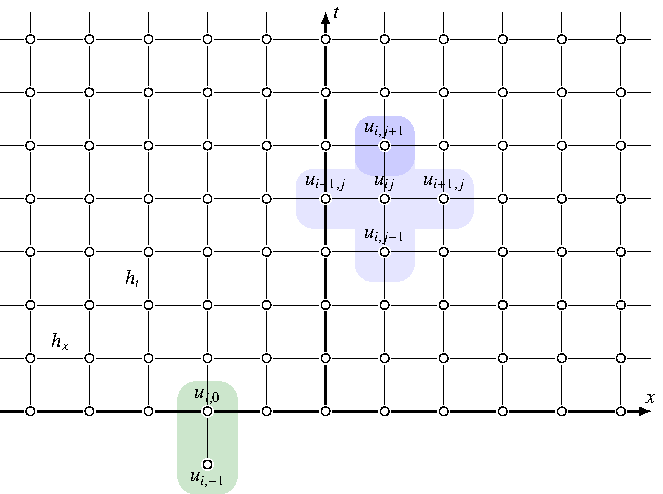
\includegraphics{chapters/2/wellengl.pdf}
\caption{Gitter für die Diskretisation der Wellengleichung.
Der etwas dunkler hinterlegte Wert $u_{i,j+1}$ kann direkt aus den
Werten $u_{i-1,j}$, $u_{ij}$ und $u_{i+1,j}$ berechnet werden.
Links unten grün hinterlegt ist die Methode illustriert, wie $u_{i,-1}$
aus den Randbedingungen berechnet werden muss, damit die Wellengleichung
gelöst werden kann.
\label{skript:wellengl:grid}}
\end{figure}
Die Wellengleichung
\index{Wellengleichung}
\[
\begin{aligned}
\frac{\partial^2u}{\partial t^2}
&=
\frac{\partial^2u}{\partial x^2}
&&\text{auf $\Omega=\{(x,t)\,|\, x\in\mathbb R\wedge t>0\}$}
\\
u(x,0)&=f(x)
&&\text{für $x\in\mathbb R$}\\
\frac{\partial u}{\partial t}(x,0)&=g(x)
&&\text{für $x\in\mathbb R$}
\end{aligned}
\]
wird von der allgemeinen Theorie \cite{skript:pde} als hyperbolische
lineare
partielle Differentialgleichung zweiter Ordnung klassifiziert.
\index{hyperbolisch}
Unter milden Voraussetzungen an die Anfangsbedingungen $f(x)$ und $g(x)$
existiert eine eindeutig bestimmte Lösung, die mit dem Formel von
d'Alembert gefunden werden kann.
\index{d'Alembert-Lösung}

Für die numerische Lösung wird wieder ein Gitter aus Punkten
$(ih_x, jh_t)$  mit $i\in\mathbb Z$ und $j\in\mathbb N$
(Abbildung~\ref{skript:wellengl:grid}).
Unter Verwendung der gleichen Approximationen  für die Ableitungen
können wir die Differentialgleichungen in ein lineares Gleichungssystem
\begin{equation}
\frac{1}{h_t^2}(u_{i,j+1}-2u_{ij}+u_{i,j-1})
-
\frac{1}{h_x^2}(u_{i+1,j}-2u_{ij}+u_{i-1,j})
=
0
\quad\Rightarrow\quad
u_{i,j+1}
=
2u_{ij}-u_{i,j-1}
+
\frac{h_t^2}{h_x^2}
(u_{i+1,j}-2u_{ij}+u_{i-1,j})
\label{skript:wellengleichung:dgl}
\end{equation}
umwandeln.
In dieser Form werden Werte für $t=(j+1)h_t$ aus Werten zu früheren
Zeiten berechnet.

Ausserdem müssen die Randbedingungen 
$u_{i0} = f(ih_x)$ für $i\in\mathbb Z$ erfüllt sein.
Dies reicht aber nicht, denn die Gleichungen
\eqref{skript:wellengleichung:dgl}
brauchen für die Berechnung von $u_{i,1}$ die Werte $u_{i,-1}$, die gar
nicht definiert sind.
Wir können aber die Ableitung nach $t$ zur Zeit $t=0$ durch einen
Differenzenquotienten
\[
\frac{\partial u}{\partial t}(ih_x,0)
\simeq
\frac{u_{i0}-u_{i,-1}}{h_t}
\qquad
\Rightarrow
\qquad
u_{i,-1} = u_{i0} -h_t g(ih_x,0)
\]
approximieren und damit einen Werte für $u_{i,-1}$ aus den Randbedingungen
ermitteln.
Dies ist in Abbildung~\ref{skript:wellengl:grid} grün hinterlegt illustriert.
Erneut haben wir es geschafft, das Problem, eine Lösung der partiellen
Differentialgleichung zu finden, auf ein lineares Gleichungssystems
zurückzuführen.

\subsubsection{Wärmeleitungsgleichung}
\begin{figure}
\centering
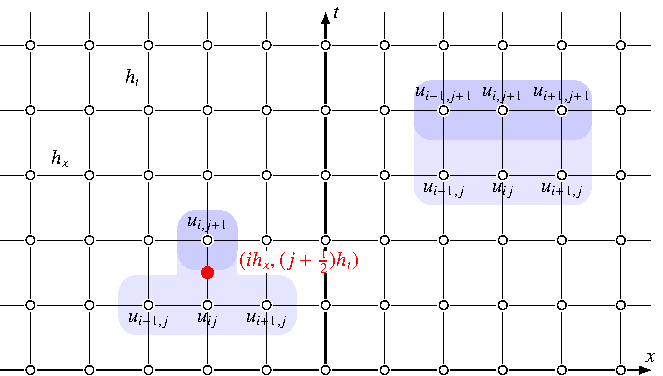
\includegraphics{chapters/2/waerme.pdf}
\caption{Gitter zur Diskretisation der Wärmeleitungsgleichung.
Oben rechts sind die sechs Gitterpunkte hervorgehoben, mit denen
die Gleichungen für das implizite Verfahren aufgestellt werden
können.
Etwas dunkler hinterlegt die unbekannten Variablen.
Links unten das nicht ganz exakte Verfahren, weil des die erste
Ableitung nach der Zeit $t$ an der Stelle $(ih_x,(j+\frac12)h_t)$
(rot eingezeichnet)
verwendet.
Die Randpunkte bei $i=\pm n$ sind nicht eingezeichnet, da damit gleich
umgegangen wird wie beim Poisson-Problem in Abbildung~\ref{skript:poisson:grid}.
\label{skript:waerme:grid}}
\end{figure}
Die Wärmeleitungsgleichung
\[
\begin{aligned}
\frac{\partial u}{\partial t}
&=
\kappa
\frac{\partial^2 u}{\partial x^2}
&&\text{in $\Omega = \{(x,t)\,|\, x\in[-1,1]\wedge t>0\}$}
\\
u(x,0)&=f(x)
&&\text{für $x\in[-1,1]$}
\\
u(-1,t)&=g_{-1}(t)
&&\text{für $t>0$}\\
u(1,t)&=g_{1}(t)
&&\text{für $t>0$}
\end{aligned}
\]
wird von der allgemeinen Theorie \cite{skript:pde} als parabolische
lineare partielle Differentialgleichung klassifiziert, sie hat
unter milden Anforderungen an $f(x)$ immer eine glatte Lösung.

Für die numerische Lösung verwenden wir wieder ein Gitter, diesmal bestehend
aus den Punkten $(x_i, t_j)=(ih_x, jh_t)$ mit $-n \le i \le n$ und
$j\in\mathbb N$, mit $h_x=1/n$ (Abbildung~\ref{skript:waerme:grid}).
Direkte Anwendung der Approximation der Ableitungen durch
Differenzenquotienten liefert
\begin{equation}
\frac{\partial u}{\partial t}(x_i,t_j)
\simeq
\frac{u_{i,j+1}-u_{ij}}{h_t}
=
\kappa
\frac{\partial^2u}{\partial x^2}(x_i,t_j)
\simeq
\kappa
\frac{u_{i+1,j}-2u_{ij}+u_{i-1,j}}{h_x^2}.
\end{equation}
Dies lässt sich nach $u_{i,j+1}$ auflösen:
\[
u_{i,j+1}
=
u_{ij}
+
\frac{\kappa h_t}{h_x^2} (u_{i+1,j}-2u_{ij}+u_{i-1,j}).
\]
Diese Gleichungen bestimmen explizit die Werte $u_{i,j+1}$ aus früheren Werten
$u_{ij}$, man nennt dies ein explizites Verfahren.

Die Randbedingungen geben uns Anfangswerte für $j=0$ und Randwerte
für $i=\pm n$, nämlich
\begin{equation}
\begin{aligned}
u_{i0} &= f(ih_x)&&\text{für $-n<i<n$}\\
u_{-n,j} & g_{-1}(jh_t)&&\text{für $j>0$}\\
u_{n,j} & g_{1}(jh_t)&&\text{für $j>0$.}
\end{aligned}
\label{skript:waerme:rand}
\end{equation}

Allerdings sind diese Approximationen nicht ganz konsistent.
Die Approximation für die erste Ableitung nach $t$ an der Stelle
$(x_i,t_j)$ ist eigentlich eher repräsentativ für den Punkt
$(x_i,t_j+\frac12h_t)$, wie dies in Abbildung~\ref{skript:waerme:grid}
{\color{red}rot}
angedeutet ist.
Eine besser Diskretisation der Wärmeleitungsgleichung bekommen wir daher,
wenn wir die Approximationen für die zweiten Ableitungen nach $x$ an
den Stellen $(x_i,t_j)$  und $(x_i,t_{j+1})$ mitteln. 
Die lineare Gleichung wird damit zu
\begin{equation}
\frac{u_{i,j+1}-u_{ij}}{h_t}
=
\frac12\biggl(
\frac{u_{i+1,j+1}-2u_{i,j+1}+u_{i+1,j+1}}{h_x^2}
+
\frac{u_{i+1,j}-2u_{ij}+u_{i+1,j}}{h_x^2}
\biggr).
\label{skript:waerme:implizit}
\end{equation}
Dies ist zusammen mit den bereits formulierten Randbedingungen
\eqref{skript:waerme:rand}
immer noch ein lineares Gleichungssystem.
Die Werte $u_{i,j+1}$ lassen sich jetzt nicht mehr so einfach
explizit ableiten, stattdessen hat das lineare Gleichungssystem
\eqref{skript:waerme:implizit}
in jeder Gleichungen drei verschiedene Variablen $u_{i,j+1}$,
die durch diese Gleichungen implizit gegeben sind.
Man nennt dies ein implizites Verfahren.
\index{implizites Verfahren}
Leider führt dieses sogenannte Leapfrog-Verfahren zu einem numerischen
Stabilitätsproblem, dem Computational Mode, welches in
Kapitel~\ref{chapter:learning} etwas ausführlicher dargestellt wird.

\subsection{Basisfunktionen}
Lineare Differentialgleichungen haben die Eigenschaft, dass 
mit zwei Lösungen auch deren Linear\-kombinationen wieder Lösungen sind.
In der Theorie der gewöhnlichen linearen Differentialgleichungen endlicher
Ordnung geben die Koeffizienten der Linearkombination die nötige Flexibilität,
die Anfangsbedingungen zu erfüllen.
Dasselbe gilt auch für partielle Differentialgleichungen, mit dem Unterschied
allerdings, dass es meinstens unendlich viele linear unabhängige Lösungen
gibt.
Ist $L$ ein linearer Differentialoperator und $u_k$, $k\in\mathbb N$, eine
Familie von Lösungen der Gleichung $Lu=0$,
dann lässt sich im besten Fall jede andere Lösung $u$ in einem noch
zu definierenden Sinn beliebig genau durch Linearkombinationen
\[
u=\sum_{k\in\mathbb N} a_ku_k
\]
approximieren.
Wir verzichten darauf, auf diese Details der Approximation einzugehen.

Bei einer nichtlinearen Differentialgleichung ist es sicher nicht
mehr möglich, Lösungen durch Linearkombination anderer Lösungen
zu bilden.
Aber es spricht nichts dagegen, dass es eine Familie $u_k$, $k=1,\dots,N$,
von Funktionen gibt, mit der man Lösungen genügend genau approximieren
kann.

\subsubsection{Die Potenzreihenmethode}
Diese Idee liegt zum Beispiel der Potenzreihenmethode zu Grunde.
Dabei nimmt man an, dass die Lösung einer Differentialgleichung als
Linearkombination der Potenzfunktionen $u_k(x)=x^k, k=0\dots,N$,
approximiert werden kann.
Als Beispiel betrachten wir die Differentialgleichung
\[
y''=-\lambda y.
\]
Eine Potenzfunktion $u_k(x)=x^k$ ist offensichtlich keine Lösung.
Man kann aber die Lösung als eine Linearkombination
der Potenzfunktionen
\[
y(x)
=
a_0+a_1x+a_2x^2+a_3x^3+\dots
\]
ansetzen und in die Differentialgleichung einsetzen.
Man erhält
\[
2\cdot 1 \cdot a_2
+
3\cdot 2 \cdot a_3x
+
4\cdot 3 \cdot a_4x^2
+
\dots
=
-\lambda(
a_0+a_1x+a_2x^2+a_3x^3+\dots).
\]
Man liest daraus die Gleichungen für die Koeffizienten $a_k$ ab:
\begin{equation*}
\left.
\begin{aligned}
2\cdot 1\cdot a_2&=-\lambda a_0\\
3\cdot 2\cdot a_3&=-\lambda a_1\\
4\cdot 3\cdot a_4&=-\lambda a_2\\
5\cdot 4\cdot a_5&=-\lambda a_3\\
&\;\;\vdots
\end{aligned}
\quad
\right\}
\qquad\Rightarrow\qquad
\left\{
\quad
\begin{aligned}
a_{2k}  &=(-1)^k\frac{\lambda^k}{ 2k!   }a_0\\
a_{2k+1}&=(-1)^k\frac{\lambda^k}{(2k+1)!}a_1
\end{aligned}
\right.
\end{equation*}
Man kann erkennen, dass jede Lösung die Form
\begin{align*}
u(x)
&=
a_0
\biggl(
1-\frac{(\sqrt{\lambda}x)^2}{2!} + \frac{(\sqrt{\lambda}x)^4}{4!}-\dots
\biggr)
+
\frac{a_1}{\sqrt{\lambda}}
\biggl(
\sqrt{\lambda}x
-
\frac{(\sqrt{\lambda}x)^3}{3!} + \frac{(\sqrt{\lambda}x)^5}{5!}-\dots
\biggr)
\\
&= a_0 \cos \sqrt{\lambda}x
+ \frac{a_1}{\sqrt{\lambda}} \sin\sqrt{\lambda}x
\end{align*}
hat.

\subsubsection{Erfolgsfaktoren}
Aus dem eben entwickelten Beispiel kann man einige heuristische Regeln ableiten,
wie die Funktionenfamilie $u_k$ beschaffen sein muss, damit es
durchführbar ist.
\begin{enumerate}
\item Die Ableitungen $u_k'(x)$ der Funktionen können durch
Linearkombinationen derselben ausgedrückt werden.
Im Beispiel ist $u'_k(x)=kx^{k-1}=ku_{k-1}(x)$.
\item Produkte von Funktionen $u_k(x)$ lassen sich durch Linearkombinationen
approximieren.
Im Beispiel ist $u_k(x)u_l(x)=x^kx^k = x^{k+l}=u_{k+l}(x)$.
\item Beim Einsetzen des Ansatzes in die Differentialgleichungen
entstehen algebraische Gleichungen, aus denen die Koeffizienten
bestimmt werden können.
\end{enumerate}

\subsubsection{Finite Elemente}
\begin{figure}
\centering
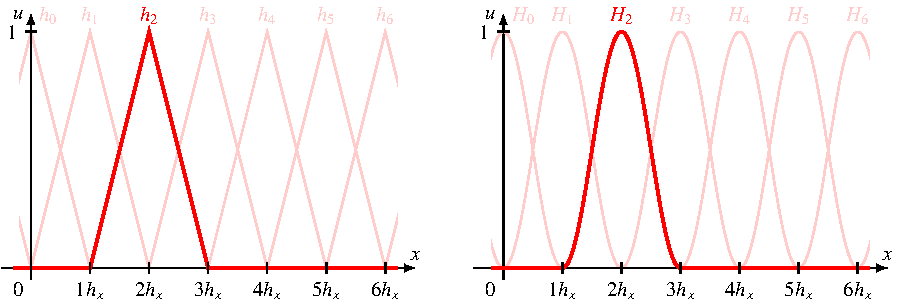
\includegraphics[width=\hsize]{chapters/2/fe.pdf}
\caption{Approximationsfunktionen $h_i(x)$ für stückweise lineare Funktionen 
$H_i(x)$ für glatte Funktionen.
\label{skript:finiteelemente}}
\end{figure}
Bei der Diskretisation in Abschnitt~\ref{section:diskretisation} wurde die
Funktion durch Werte an den Gitterpunkten ersetzt.
Für die Berechnung der Ableitung wurde die Funktion linear interpoliert.
Lineare Funktionen zwischen benachbarten Gitterpunkten können daher als
Basisfunktionen verwendet werden.
Damit die Funktionen stetig werden, kann man stückweise lineare
Funktionen
\[
h_i(x) =
\begin{cases}
0&\qquad x< (i-1)h_x\\
\frac{1}{h_x}(x-(i-1)h_x)&\qquad (i-1)h_x \le x < ih_x\\
-\frac{1}{h_x}(x-(i+1)h_x)&\qquad ih_x \le x < (i+1)h_x\\
0&\qquad x \ge (i+1)h_x
\end{cases}
\]
verwenden, die nur an einem einzigen Gitterpunkt von $0$
verschieden sind, wie in Abbildung~\ref{skript:finiteelemente} links.

Noch bessere Resultat kann man erhalten, wenn man die Funktionen
$h_i(x)$ durch geeignete glatte Funktionen $H_i(x)$ wie in
Abbildung~\ref{skript:finiteelemente} rechts ersetzt.
Diese Idee lässt sich zu einem sehr erfolgreichen numerischen
Lösungsverfahren ausbauen, der Methode der finiten Elemente.

\subsubsection{Ein etwas komplexeres Beispiel\label{subsubsection:komplexeres}}
Wir versuchen, diese Idee auf die Lösung der Gleichung von
Burgers
\begin{equation}
\frac{\partial u}{\partial t} + u\frac{\partial u}{\partial x}=0
\qquad\text{mit Randbedingung}\qquad
u(0,x)=g(x)
\label{skript:pde:burgersequation}
\end{equation}
anzuwenden.
Wir suchen $2\pi$-periodische Lösungen für ebensolche Anfangsbedingung
$u(0,x)=g(x)$.
Wie im Kapitel~\ref{chapter:fourier} dargelegt wird, sind die Funktionen
$\cos kx$ und $\sin kx$ geeignete Basisfunktionen für das skizzierte Verfahren.
Zur Vereinfachung der Rechnung verwenden wir statt der reellen Funktion
$\cos kx$ und $\sin kx$ die komplexen Exponentialfunktionen $e^{ikx}$.
Als Ansatz verwenden wir daher
\[
u(x) = \sum_{k\in\mathbb Z} c_k(t) e^{ikx}
\]
und setzen dies in die Differentialgleichung ein, die dadurch zu
\[
\sum_{k\in\mathbb Z} \dot c_k(t) e^{ikx}
=
-\sum_{j,l\in\mathbb Z} c_j(t)e^{ijx} c_l(t) le^{ilx}
=
-\sum_{j,l\in\mathbb Z} c_j(t)c_l(t) le^{i(j+l)x}
\]
wird.
Wir lesen die Gleichungen
\begin{equation}
\dot c_k(t) = -\sum_{l} lc_l(t)c_{k-l}(t)
\label{burgers:gewoedgl}
\end{equation}
für die Koeffizienten ab.
Wir haben also ein System von gewöhnlichen linearen Differentialgleichungen
erster Ordnung gefunden, und damit das partielle Differentialgleichungssystem
auf ein einfachers System reduziert.
Allerdings ist von der rechten Seite der Differentialgleichung
\eqref{burgers:gewoedgl}
nicht einmal garantiert, dass diese Summen konvergieren.

\begin{figure}
\centering
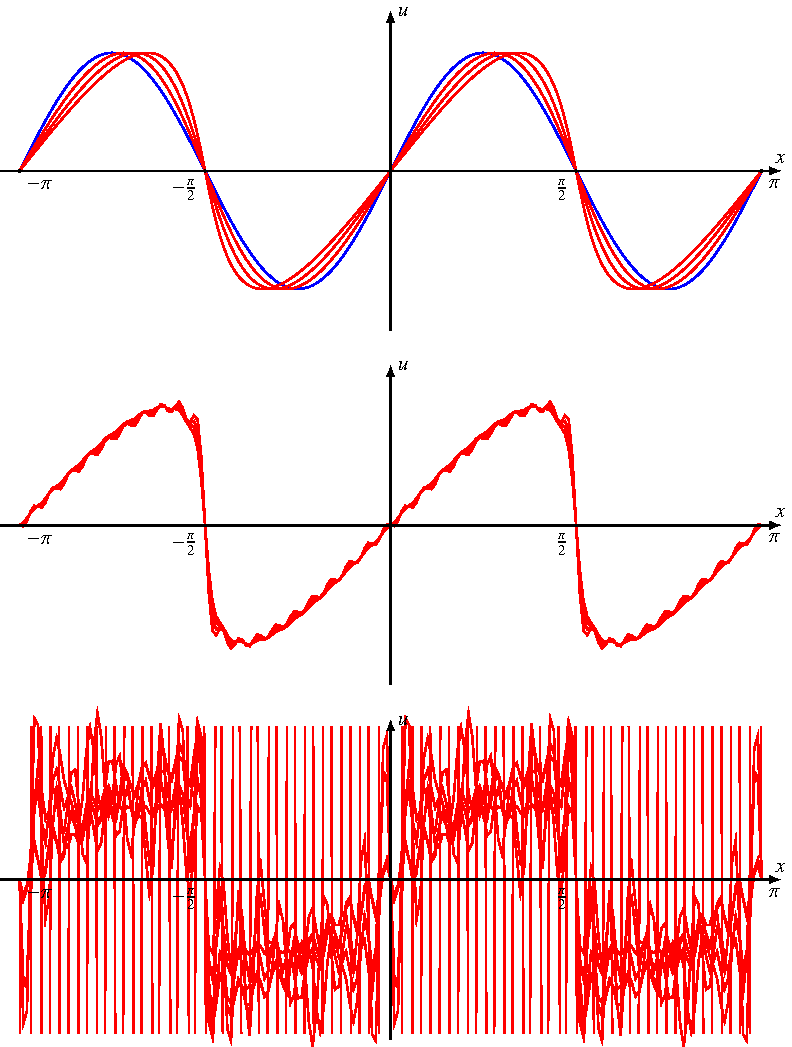
\includegraphics{chapters/2/burgfourier.pdf}
\caption{Numerische Lösung der Gleichung
\eqref{skript:pde:burgersequation}
von Burgers für die Anfangsbedingung mit Hilfe der trigonometrischen
Funktionen $\sin kx$ und $\cos kx$ als Basis.
Die Approximation ist stabil (oben), solange keine Sprungstelle auftritt,
wie dies im mittleren Graph bei $t=0.5$ passiert.
Für spätere Zeiten wird das System instabil und die berechnete Lösung
unbrauchbar (unten).
\label{skript:burgfourier}}
\end{figure}%

Für eine approximative Lösung vernachlässigen wir die Koeffizienten $c_k$
mit $|k|>N$ und berechnen die Lösungen der Differentialgleichungen
\eqref{burgers:gewoedgl} numerisch für die Anfangsfunktionen
\begin{equation}
u(0,x) = g(x) = \sin 2x.
\end{equation}
Die Resultate sind in Abbildung~\ref{skript:burgfourier} dargestellt.

Lösungen der Gleichung von Burgers können in allgemeiner Form mit
Hilfe der Methode der Charakteristiken gefunden werden \cite{skript:pde},
ein kurzer Abriss dieser Lösung wird in Abschnitt~\ref{section:burgersallg}
gegeben.
Für glatte Anfangsbedingungen beschreibt die Gleichung von Burgers eine
Welle, die sich mit einer Geschwindigkeit in $x$-Richtung bewegt, die
proportional zu $u$ ist.
Der Kamm einer Welle bewegt sich also schneller als der Sockel.
Bis zu $t=0.4$, dargestellt im obersten Bild von
Abbildung~\ref{skript:burgfourier} kann man genau dies auch in der
numerischen Lösung beobachten.

Die allgemeine Theorie sagt aber auch, dass nach genügend langer
Zeit der Kamm der Welle den Sockel überholt und sich eine Sprungstelle
zu entwickeln beginnt.
Die Sprungstelle bewegt sich mit dem Mittelwert der Grenzwerte von $u$
auf beiden Seiten der Sprungstelle.
Für die gegebenen Anfangsbedingungen entsteht zur Zeit $t=\frac12$
eine Sprungstelle an den Stellen $x=\frac{\pi}2+k\pi\mathbb Z$.
Die Lösung ist antisymmetrisch an diesen Punkten, daher bewegt sich
die Sprungstelle nicht.
Dies kann man auch aus der numerischen Lösung in
Abbildung~\ref{skript:burgfourier}
in der Mitte beobachten.
Natürlich kann eine Sprungstelle mit endlich vielen Fourier-Termen
nicht getreu wiedergegeben werden, das Gibbs-Phänomen sagt voraus,
dass sich in der Nähe der Sprungstelle grösser werdende Oszillationen
entwickeln.
Diese Oszillationen breiten sich in der numerischen Lösung rasch
über den gesamten Definitionsbereich aus.

Für grosse Zeiten verspricht die allgemeine Theorie, dass die Lösung
eine Sägezahn-ähnliche Funktion wird die gegen $0$ konvergiert.
Die numerische Lösung deutet dies an in Abbildung~\ref{skript:burgfourier}
unten, obwohl sie von den ständig anwachsend Oszillationen überdeckt werden.

Dieses Beispiel zeigt also einerseits, wie die Verwendung einer Basis
aus einer partiellen Differentialgleichung
eine gewöhnliche Differentialgleichung machen kann, die unter geeigneten
Bedingungen auch vernünftige Lösungen liefern kann.
Andererseits zeigt es auch die Grenzen dieses Vorgehens auf.

\subsection{Separation}
\index{Separation}%
\subsubsection{Motivation}
Besonders gut geeignet als Basisfunktionen sind Funktionen, die bereits
Lösungen einer vereinfachten Variante der partiellen Differentialgleichung
sind oder die die Randbedingungen leicht wiederzugeben erlauben.
Zum Beispiel kommt in den Strömungsdifferentialgleichungen häufig der
Laplace-Operator vor, also könnte es nützlich sein, als Basisfunktionen
eine Familie von Funktionen $u_n$ heranzuziehen, welche bereits Lösungen
der Gleichung $\Delta u_n=\lambda_nu_n$ sind.
In Kapitel~\ref{chapter:lorenz2} wird
gezeigt, wie man diese Idee auf das in
Abschnitt~\label{section:lorenz-modell} vorgestellte Lorenz-Modell
andwenden kann.
Wenn man dann die Lösung als Linearkombination $\sum a_nu_n$ dieser Funktionen
ansetzt, verschwinden alle Terme der Form $\Delta u_n$, was die gewöhnlichen
Differentialgleichungen für die Koeffizienten $a_n$ dramatisch vereinfachen
kann.
In diesem Abschnitt zeigen wir daher an einem Beispiel, wie solche Funktionen
gefunden werden können. 

\subsubsection{Die Separationsmethode an einem Beispiel}
Gegeben sei die Differentialgleichung
\[
\begin{aligned}
\Delta u &= \lambda u&&
\text{auf dem Gebiet $\Omega=\{ (x,y)\,|\, 0<x<a\text{ und }0<y<b\}$}
\\
\text{mit}
\qquad
u=&0&&\text{auf dem Rand $\partial\Omega$.}
\end{aligned}
\]
Das Gebiet ist ein Rechteck mit Seitenlängen $a$ und $b$.
Die Relation $\Delta u=\lambda u$ ermöglicht, jedes Vorkommen eines auf
die Funktion $u$ wirkenden Laplace-Operators durch die Multiplikation
mit $\lambda$ zu ersetzen, und damit die Differentialgleichung zu vereinfachen.

Die Separationsmethode nimmt jetzt an, dass sich die Lösung der
Differentialgleichung in der besonders einfachen Form eines Produktes
$u(x,y)=X(x)\cdot Y(y)$ finden lässt.
Setzt man diesen Separationsansatz
\index{Separationsansatz}
in die Differentialgleichung ein, erhält man
\[
\Delta u
=
\biggl(
\frac{\partial^2}{\partial x^2}
+
\frac{\partial^2}{\partial y^2}
\biggr)
X(x)\cdot Y(y)
=
X''(x)\cdot Y(y) + X(x)\cdot Y''(y)
=
\lambda X(x)\cdot Y(y).
\]
Wir interessieren uns für nicht verschwindende Lösungen, wir nehmen daher
an, dass die Funktionen $X(x)$ und $Y(y)$ nur isolierte Nullstellen haben.
Ausserhalb dieser Nullstellen ist es erlaubt, durch $X(x)\cdot Y(y)$ zu
divideren. 
Damit wird es möglich, die Variablen $x$ und $y$ zu trennen, man
erhält
\[
0
=
\frac{X''(x)\cdot Y(y) + X(x)\cdot Y''(y)}{X(x)\cdot Y(y)} - \lambda
=
\frac{X''(x)}{X(x)}
+
\frac{Y''(y)}{Y(y)}
-
\lambda
\qquad\Rightarrow\qquad
\frac{X''(x)}{X(x)}=-\frac{Y''(y)}{Y(y)}+\lambda.
\]
Die linke Seite der Gleichung hängt nur von $x$ ab, die rechte nur von $y$.
Ändert man $x$ während man $y$ konstant hält, dann kann sich die rechte
Seite nicht ändern, die linke muss daher auch konstant sein.
Wenn aber die linke Seite eine Konstante ist, dann muss auch die rechte
eine Konstante sein. 
Es gibt also eine vorerst noch unbekannte Konstante $\mu$, so dass
die Funktionen $X(x)$ und $Y(y)$ die Differentialgleichungen
\begin{equation}
X''(x) = -\mu X(x)
\qquad\text{und}\qquad
Y''(y) = (\lambda+\mu)Y(y)
\label{skript:separation:gleichungen}
\end{equation}
erfüllen.
Mögliche Werte für $\mu$ werden sich daraus ergeben, ob die
Differentialgleichungen überhaupt lösbar sind, oder ob
sich die gegebenen Randbedinungen erfüllen lassen.

Wir lösen die Differntialgleichungen~\eqref{skript:separation:gleichungen}
so, dass auch die Randbedingungen $u=0$ auf $\partial\Omega$ erfüllt sind.
Für die Funktionen $X(x)$ und $Y(y)$ bedeutet dies:
\[
\begin{aligned}
X(0)&=0,&&& Y(0) &= 0,\\
X(a)&=0,&&& Y(b) &= 0.
\end{aligned}
\]
Die linearen Differntialgleichungen~\eqref{skript:separation:gleichungen}
haben Exponentialfunktionen oder trigonometrische Funktionen als
Lösungen.
Da sich mit Exponentialfunktionen die Randbedingungen ohnehin nicht
einhalten lassen, suchen wir Lösungen als trigonometrische Funktionen.
Da $X(0)=0$ und $Y(0)=0$ gilt, müssen die Lösungen Sinus-Funktionen sein,
wir nehmen daher an, dass $X(x)=\sin \kappa x$ und $Y(y)=\sin \nu y$.
Für diese Funktionen gilt
\[
\begin{aligned}
X''(x) &= -\kappa^2\sin \kappa x = -\kappa^2 X(x)
&&\text{und}&
Y''(y) &= -\nu^2\sin \nu x = -\nu^2 Y(y).
\end{aligned}
\]
Die Randbedingungen am rechten Rand sind
\[
\begin{aligned}
X(a) = \sin \kappa a = 0
&
Y(b) = \sin \nu b = 0.
\end{aligned}
\]
Da die Sinus-Funktion ihre Nullstellen genau bei den ganzzahligen Vielfachen
von $\pi$ hat, schliessen wir, dass $\kappa a = k\pi$ und $\nu b = l\pi$
mit $k,l\in\mathbb Z$ gilt.
Die Lösungen sind daher von der Form
\[
\begin{aligned}
X(x) &= \sin \frac{xk\pi}{a}
&
&\text{und}
&
Y(y) &= \sin\frac{yl\pi}{b}.
\end{aligned}
\]
Wir bekommen so die Familie der Lösungsfunktionen
\[
u_{kl}(x,y) = \sin \frac{xk\pi}{a} \sin\frac{yl\pi}{b}.
\]
Wir berechnen auch noch die Werte von $\mu$ und $\lambda$:
\begin{align*}
X''(x)
&=
-\mu X(x) = -\frac{k^2\pi^2}{a^2}
\\
\Delta u_{kl}
&=
-\frac{k^2\pi^2}{a^2} u_{kl}
-\frac{l^2\pi^2}{b^2} u_{kl}
=
-\biggl(\frac{k^2}{a^2}+\frac{l^2}{b^2}\biggr)\pi^2 u_{kl}
=
\lambda  u_{kl}
&&\Rightarrow&
\lambda_{kl} = - \biggl(\frac{k^2}{a^2}+\frac{l^2}{b^2}\biggr)\pi^2.
\end{align*}
Nur ein diskrete Menge von Zahlenwerten $\mu$ sind also möglich, und nur 
für eine diskrete Menge von Eigenwerten $\lambda$ ist die ursprüngliche 
Differentialgleichung überhaupt lösbar.

Damit haben wir eine Familie $u_{kl}$, $k,l\in\mathbb Z$ von Funktionen
gefunden, die Lösungen der Differentialgleichung
$\Delta u_{kl}=\lambda_{kl} u_{kl}$ sind.
Das Anfangs gesteckte Ziel ist erreicht.

\subsubsection{Verallgemeinerungen}
Das Beispiel deutet auch an, wie die Methode verallgemeinert werden kann.
\begin{enumerate}
\item
Wenn möglich, wähle ein Koordinatensystem, mit welchem das Definitionsgebiet
einfach beschrieben werden kann.
Formuliere die Differentialgleichung in diesen Koordinaten.
Darstellungen des Laplace-Operator für fast alle wichtigen Koordinatensysteme
können zum Beispiel in guten Formelsammlungen gefunden werden.
\item
Separationsansatz: setze die Lösung als Produkt von Funktionen an,
jeweils von nur einer Koordinate abhängen, also
$u(x,y)=X(x)\cdot Y(y)$ in einem $x$-$y$-Koordinatensystem.
\item
Setze den Ansatz in die Differentialgleichung ein und versuche die
Variablen zu trennen. 
Gesucht ist eine Gleichung, deren linke Seite nur von einer Variablen
abhängt, die rechte nur von allen anderen.
Wie im Beispiel folgt, dass beide Seiten konstant sein müssen.
Damit hat man das Problem darauf reduziert, eine gewöhnliche
Differentialgleichung für eine Funktion der einen Variable zu lösen.
Integrationskonstation, die in der Lösung der gewöhnlichen
Differentialgleichung immer auftreten wird, können oft mit Hilfe
eines Teils der Randbedingungen eliminiert werden.
\item
Durch Iteration von Schritt~3 können Teillösungen $u_n$ gefunden werden,
die von den Konstanten abhängen, die bei der Separation eingefügt werden
müssen.
\end{enumerate}

